Goでは2つの関数が予約されています:\texttt{init}関数(すべての\texttt{package}で使用できます)と\texttt{main}関数(\texttt{package main}でしか使用できません)です。この2つの関数は定義される際いかなる引数と戻り値も持ちません。\texttt{package}のなかで複数の\texttt{init}関数を書いたとしても、もちろん可読性か後々のメンテナンス性に対してですが、\texttt{package}の中では各ファイルに一つだけの\texttt{init}関数を書くよう強くおすすめします。

Goのプログラムは自動で\texttt{init()}と\texttt{main()}をコールしますので、どこかでこの2つの関数をコールする必要はありません。各\texttt{package}の\texttt{init}関数はオプションです。しかし\texttt{package main}は必ず一つ\texttt{main}関数を含まなければなりません。

プログラムの初期化と実行はすべて\texttt{main}パッケージから始まります。もし\texttt{main}パッケージが他のパッケージをインポートしていたら、コンパイル時にその依存パッケージがインポートされます。あるパッケージが複数のパッケージに同時にインポートされている場合は、先にその他のパッケージがインポートされ、その後このパッケージの中にあるパッケージクラス定数と変数が初期化されます。次にinit関数が(もしあれば)実行され、最後に\texttt{main}関数が実行されます。以下の図で実行過程を詳しくご説明しています。

\begin{figure}[H]
  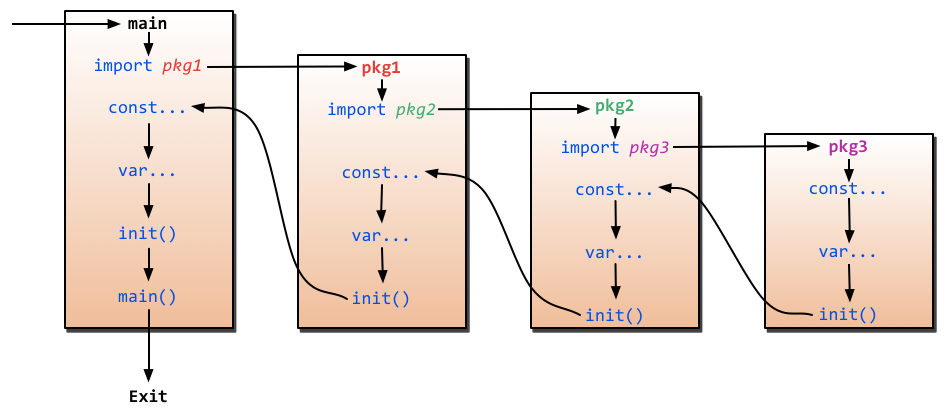
\includegraphics[width=14cm]{2.3.init.png}
   \label{図2.6}
   \caption{main関数によるパッケージのインポートと初期化過程の図}
\end{figure}
